\subsection{Problem and Motivations}

\begin{frame} \frametitle{Problem and Motivations}

\begin{itemize}
\item Given an initial shape $\mathcal{I}$, a goal shape $\mathcal{G}$ and the mechanical constraints
\item Problem: self-reconfigure the robot from shape $\mathcal{I}$ to $\mathcal{G}$
\begin{center}
	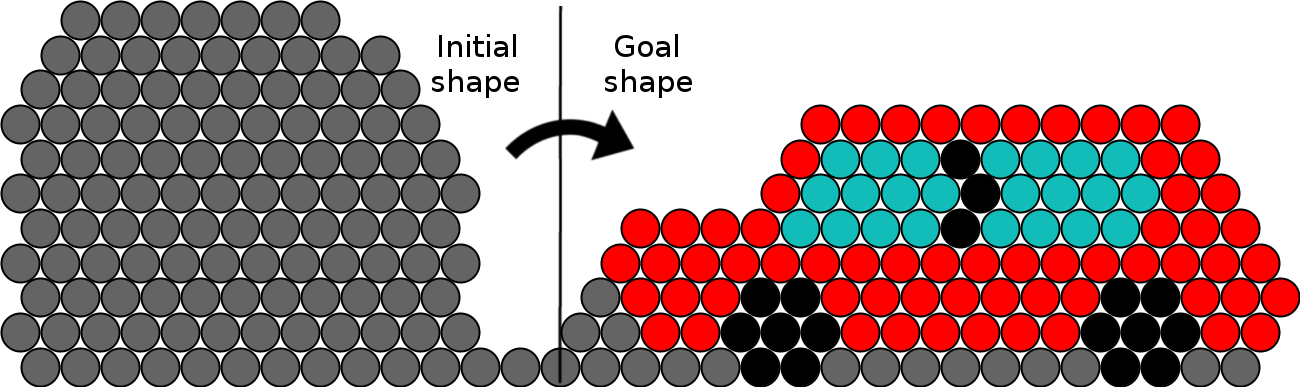
\includegraphics[width=0.6\linewidth]{fig/reconfiguration/car.png}
\end{center}
\item Challenge: Distributed coordination
\begin{itemize}
	\item Effectiveness: reach $\mathcal{G}$
	\begin{itemize}
		\item Prevent collisions
		\item Prevent deadlock %(mechanical constraints) 
	\end{itemize}
	\item Efficiency
	\begin{itemize}
		\item Execution time	
		\item Motion
		\item Communication	
	\end{itemize}
\end{itemize}
\item Motivation: programmable matter
\end{itemize}

\end{frame}

\subsection{System Model and Assumptions}

\noLogo{
\begin{frame} \frametitle{System Model and Assumptions}

\begin{itemize}
\item Hexagonal lattice:
\begin{itemize}
	\item Every module knows its coordinates and its neighbor ones
\end{itemize}
\item Communications:
\begin{itemize}
	\item Asynchronous
	\item Neighbor-to-neighbor only
\end{itemize}
\item Motions:
\begin{itemize}
	\item Asynchronous
	\item Mechanical constraints
	\item No presence sensor: prevent collisions using communications
\end{itemize}
\item Failure-free environment (modules, communications, motions, lattice)
\item Every module stores a complete representation of $\mathcal{G}$
\end{itemize}
\begin{figure}
\vspace{-0.2cm}
\centering
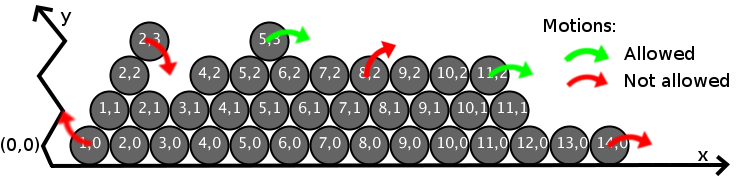
\includegraphics[width=\linewidth]{fig/reconfiguration/model}
\label{fig:model}
\end{figure}
\end{frame}
}


\subsection{Related Work}

{
\newcommand{\lenMinusOne}{0.08\linewidth}
\newcommand{\lenZero}{0.09\linewidth}
\newcommand{\lenOne}{0.12\linewidth}
\newcommand{\lenTwo}{0.14\linewidth}
\newcommand{\lenThree}{0.18\linewidth}
\newcommand{\lenFour}{0.22\linewidth}
\newcommand{\lenFive}{0.27\linewidth}
\newcommand{\lenSix}{0.28\linewidth}

\noLogo{
\begin{frame} \frametitle{Related Work}
{
\scriptsize
\begin{center}
\begin{tabular}{|C{\lenFive}|C{\lenThree}|C{\lenTwo}|C{\lenSix}|}
	\hline
	Cite & Shapes & Constraints on module movement & Collision and deadlock avoidance \\
	\hline
	\cite{walter2000distributed} & \bad{chain to chain} & \bad{relaxed} & centralized pre-computation, synchronous rounds\\
	\hline
	\cite{walter2005algorithms,bateau2012increasing} & \bad{chain to 2D} & \bad{relaxed} & centralized pre-computation, synchronous rounds\\
	\hline
	%lakhlef2015fast
	\cite{lakhlef2015energy} & \bad{chain to square} & \bad{relaxed and very-relaxed} & predefined shape construction\\
	\hline
	\cite{lakhlef2014optimization} & \bad{arbitrary to square} & \bad{relaxed} & predefined shape construction\\
	\hline
	%wong2013deterministic
	\cite{wong2015unpacking} & \bad{compact 2D to chain} & \bad{relaxed} & touch sensors, synchronous rounds, single direction \\
	\hline
	\cite{de2006scalable} & \good{2D} & \bad{relaxed} &  \\
	\hline
	\cite{rubenstein2014programmable} & \good{horizontal 2D compact} & \bad{very relaxed} & collision allowed (swarm robotic) \\
	\hline
\end{tabular}
\end{center}

\begin{center}
\begin{tabular}{|C{\lenFive}|C{\lenThree}|C{\lenTwo}|C{\lenSix}|}
	\hline
	Contribution: C2SR  & \good{vertical 2D compact} & \good{strong} & messages, single direction\\
	\hline
\end{tabular}
\end{center}
}
\end{frame}
}
}


\subsection{Contribution: The Cylindrical-Catoms Self-Reconfiguration (C2SR) Algorithm}

\subsectionOutlineFrame

\subsubsection{Shape Admissibility Conditions}

\noLogo{
\begin{frame} \frametitle{Shape Admissibility Conditions}
% both initial ang goal shapes at the same time
\begin{itemize}
\item $|\mathcal{I}| \geq |\mathcal{G}|$
\item $\mathcal{I}$ and $\mathcal{G}$ are next to each other and share some bottom cells
\item No hole
\item Wide peripheral path with no narrow passage
\end{itemize}
\begin{figure}
\centering
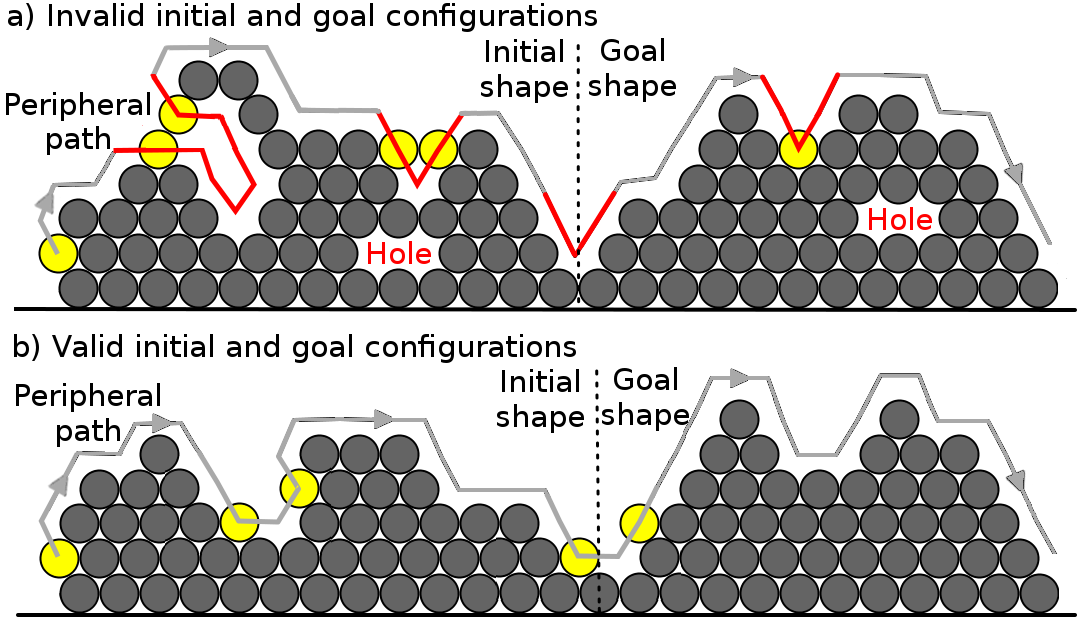
\includegraphics[width=0.75\linewidth]{fig/reconfiguration/admissibility}
\end{figure}
\end{frame}
}

\subsubsection{Algorithm}

\noLogo{
	\begin{frame} \frametitle{C2SR at a Glance}
	\begin{itemize}
	\item Stream of moving modules on the periphery 
	%(CW or CCW)
	\item Maintains an empty cell between moving modules
	\item Layer-by-layer deconstruction/construction (for shapes with only continuous horizontal layers)
	\item Decentralized with local interactions only ($ < 5$ hops)
	\begin{itemize}
		\item Communications with modules geographically around the next position in the stream
	\end{itemize}
	\end{itemize}
	
	\begin{center}
		\begin{columns}[c]
			\begin{column}{.55\textwidth}
				\centering
				\href{run:videos/54-car.avi?autostart&loop}{\adjincludegraphics[width=\linewidth]{videos/54-car.jpg}}
			\end{column}
			\begin{column}{.45\textwidth}
				\centering
				\adjincludegraphics[width=\linewidth,valign=c]{fig/reconfiguration/state-diagram}
			\end{column}
		\end{columns}
	\end{center}	
	\end{frame}
}

\subsection{Evaluation}

\subsubsection{Experimental Setup}

\subsectionOutlineFrame

\noLogo{
\begin{frame} \frametitle{Experiment Setup}

\begin{itemize}
\item VisibleSim
\item Parameters (unless otherwise mentioned)
\begin{itemize}
\item 4 shapes with different scale from $10^1$ to $10^4$ modules
\item Communication rate $\rightarrow \mathcal{N}(38.9 kpbs,389bps)$\ \ \ ($[3ms,8ms]$)
\item Motion speed $\rightarrow \mathcal{N}(1.88 mm \cdot s^{-1},0.0188 mm \cdot s^{-1})$ \ \ \ ($[273ms,285ms]$)
\end{itemize}
\item Evaluation criteria
\begin{itemize}
\item Effectiveness
\item Efficiency
\begin{itemize}
\item Time
\item Motion
\item Communication
\end{itemize}
\end{itemize}
\end{itemize}

%~\\

\begin{columns}[b]
\begin{column}{.24\textwidth}
\centering
\adjincludegraphics[width=\linewidth,height=0.9\linewidth,valign=t]{fig/reconfiguration/car-9644.png}\\
Car
\end{column}
\begin{column}{.24\textwidth}
\centering
\adjincludegraphics[width=\linewidth,height=0.9\linewidth,valign=t]{fig/reconfiguration/flag-12407.png}\\
Flag
\end{column}
\begin{column}{.24\textwidth}
\centering
\adjincludegraphics[width=\linewidth,height=0.9\linewidth,valign=t]{fig/reconfiguration/magnet-10220.png}\\
Magnet
\end{column}
\begin{column}{.24\textwidth}
\centering
\adjincludegraphics[width=\linewidth,height=0.9\linewidth,valign=t]{fig/reconfiguration/pyramid-8033.png}\\
Pyramid
\end{column}
\end{columns}
\end{frame}
}

\subsubsection{Simulation Results}

\definecolor{remarkColor}{RGB}{20,91,155}  % femtost darkblue
\renewcommand{\ResultsScaleFactor}{1}

\newcommand{\NumberExecutionAd}{
\begin{textblock*}{0.5\paperwidth}(0\paperwidth,0.925\paperheight)
\small
*Each point: 10 executions
\end{textblock*}
}

\noLogo{
\begin{frame} \frametitle{Effectiveness: C2SR in Video}

\begin{center}
	
\href{run:videos/57-car1073-x3.avi?autostart&loop}{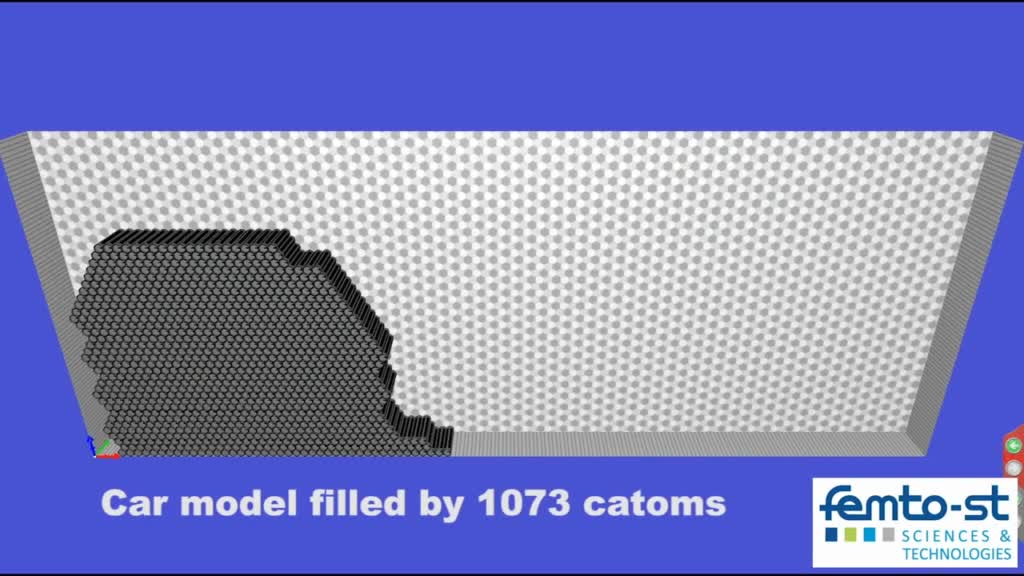
\includegraphics[width=0.95\linewidth]{videos/57-car1073-x3.jpg}}
\end{center}
\vspace{-0.25cm}
*Speed: x3
\end{frame}
}

\newcommand{\localOutline}[3]{}

\begin{frame} \frametitle{Execution Time ($\pm$ standard-deviation)}

\centering
\begin{tikzpicture}[remember picture,overlay,baseline=-2mm]
\node (image) at (0,-1cm) {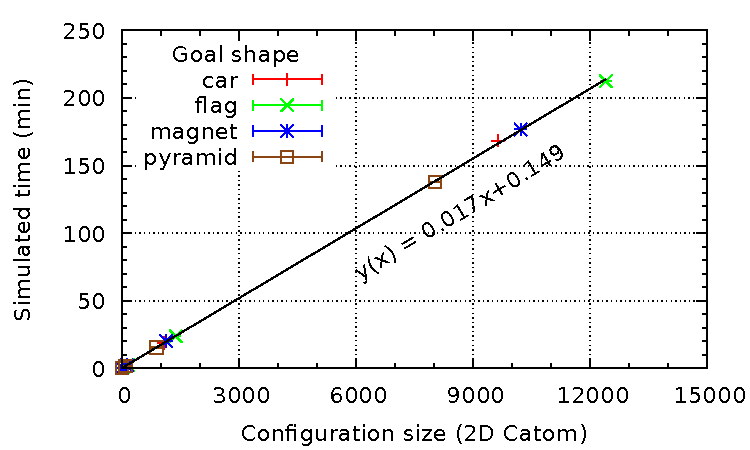
\includegraphics[width=\ResultsScaleFactor\linewidth]{./fig/reconfiguration/time}};
\draw[line width=1pt,remarkColor,<-] (2,-1) -- (2.5,-1.50)  node[label={[fill=white,align=center]Linear in the \# modules,\\highly predictable\\ $\frac{1}{0.017} \approx  1$ goal cell/second.}, yshift=-1.825cm, xshift=0.25cm] {};

%59$ goal cell/minute
\end{tikzpicture}
\NumberExecutionAd
\end{frame}

\begin{frame} \frametitle{Average Total Number of Motions ($\pm$ standard-deviation)}
\centering
\begin{tikzpicture}[remember picture,overlay,baseline=-2mm]
\node (image) at (0,-1cm) {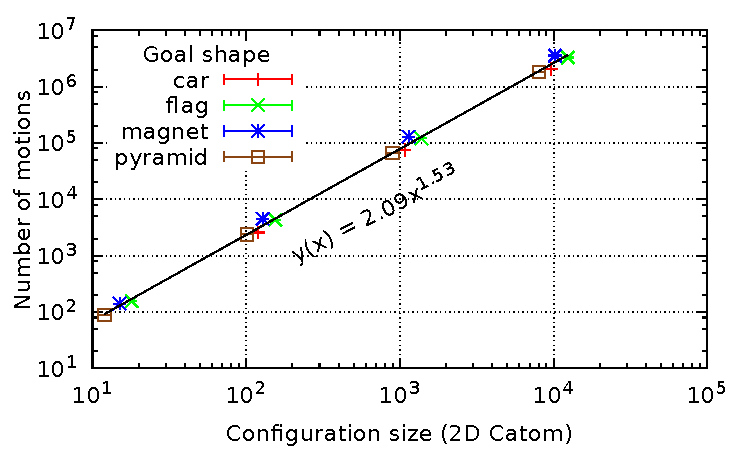
\includegraphics[width=\ResultsScaleFactor\linewidth]{fig/reconfiguration/motion}};
\draw[line width=1pt,remarkColor,<-] (1,-1) -- (1.5,-1.50)  node[label={[align=center]Polynomial in the \# modules\\Highly predictable}, yshift=-1.25cm, xshift=0.5cm] {};
\end{tikzpicture}
\NumberExecutionAd
\end{frame}

\begin{frame} \frametitle{Average Number of Messages per Catom ($\pm$ min/max)}

\centering
\begin{tikzpicture}[remember picture,overlay,baseline=-2mm]

\node (image) at (0,-1cm) {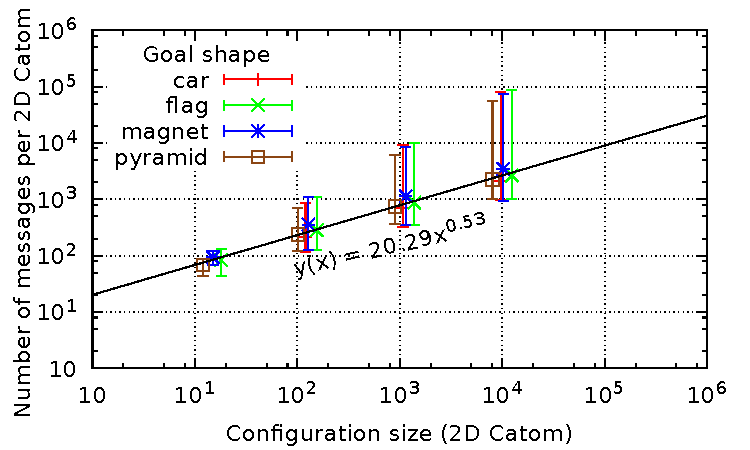
\includegraphics[width=\ResultsScaleFactor\linewidth]{fig/reconfiguration/message-individual}};

\draw[line width=1pt,remarkColor,<-] (0.5,-1.5) -- (1,-2.0)  node[label={[align=center]Polynomial in the \# modules\\Highly predictable}, yshift=-1.25cm, xshift=0.5cm] {};

\draw<2>[line width=1pt,remarkColor,->] (1,1.5) -- (0.5,0.5){};
\draw<2>[line width=1pt,remarkColor,->] (1,1.5) -- (-0.75,-0.25){};
\draw<2>[line width=1pt,remarkColor,->] (0.7,1.6) -- (1.7,0.9){};
\draw<2>[line width=1pt,remarkColor] (1.5,1) node[label={[fill=white,align=center]A few modules (at most)\\send a lot more messages}, yshift=0.25cm, xshift=0cm] {};

\node<3> (image) at (0,-1cm) {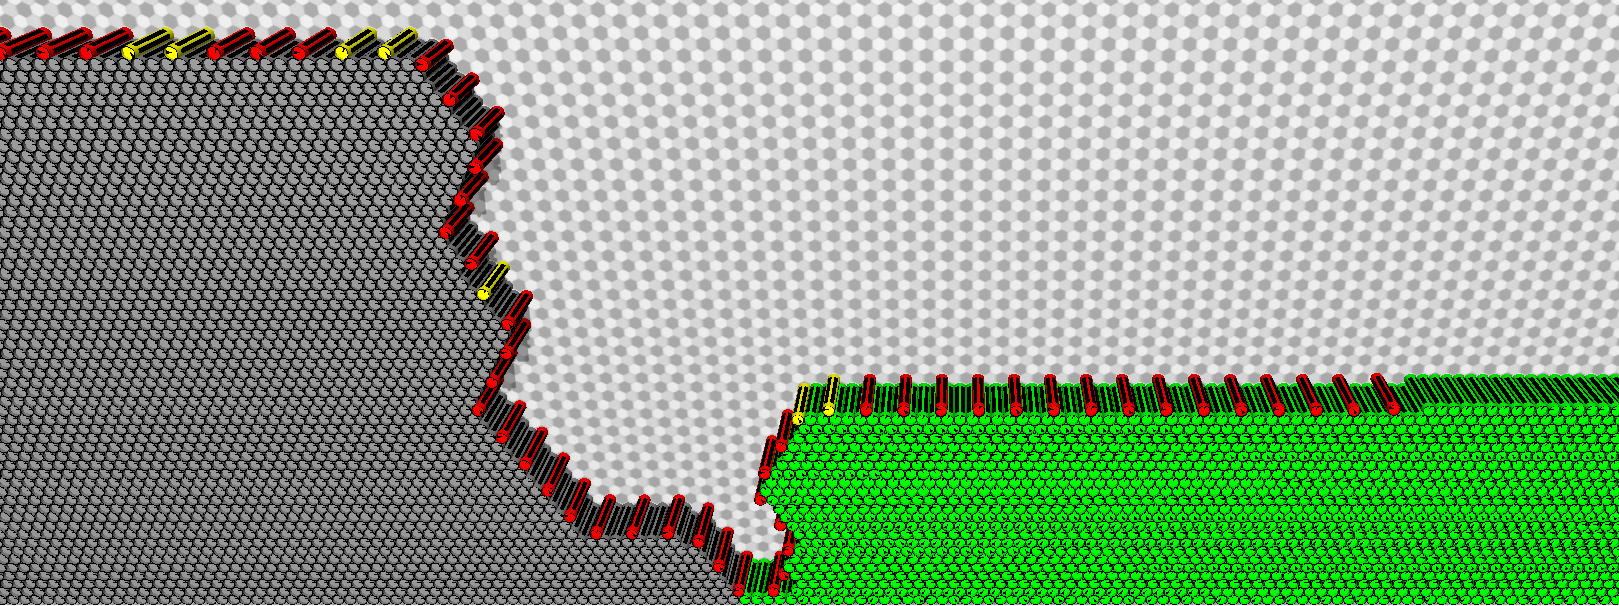
\includegraphics[width=\ResultsScaleFactor\linewidth]{fig/reconfiguration/parallelism}};
\draw<3>[draw, line width=2pt,remarkColor,label={[xshift=1.0cm, yshift=-0.15cm,align=center]\textcolor{remarkColor}{Communication hotspot}}] (-0.25,-2.5) ellipse (1 and 1);
\node<3>[fill=white] at ($(-0.25,-2)+(75:2 and 1)$) {\textcolor{remarkColor}{Communication hotspot}};
\end{tikzpicture}
\NumberExecutionAd
\end{frame}


\subsection{Conclusion}

\begin{frame}
\frametitle{Conclusion}
\begin{itemize}
	\item The Cylindrical-Catoms Self-Reconfiguration (C2SR) Algorithm
	\begin{itemize}
		\item Effective: tested on different types of shapes
		\item Scalable: tests with more than 10,000 modules
		\item Nice properties:
		\begin{itemize}
		%	\item Local and controlled communications
			\item Execution time seems linear in the size of the goal shape
			\item Highly predictable: number of motions and messages
		\end{itemize}
	\end{itemize}
	\item Limits
	\begin{itemize}
		\item Correctness and performance only shown experimentally
		\item 2D systems only
	\end{itemize}
\end{itemize}
\end{frame}